\chapter{Appendix}



\section{Linear Regression}



Calibration can be done through different statistical methods and the most popular approach is Linear Regression method. In statistics, the term regression is used to describe a group of methods that summarize the degree of association between one variable (or set of variables) and another variable (or set of variables) \cite{Burke}. Linear Regression establishes relationship between two variables one is the independent variable which will be on the $x$ axis and the dependent variable in the $y$ axis by drawing a straight line. If there are many observations and is plotted as a scatter plot then a line called as regression line as in the figure \ref{LRM} could be drawn through it by the Least Square method. 


\begin{figure}[h]
    \begin{center}
    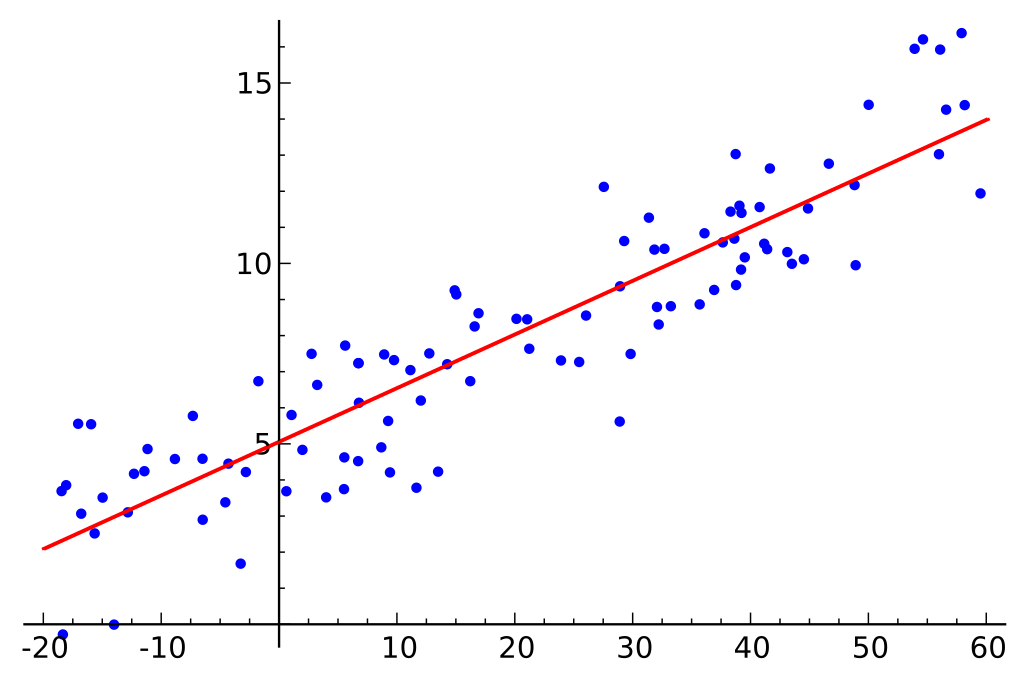
\includegraphics[scale=0.25]{./images/figure9.png} 
    \end{center}
    \caption{Linear regression model \cite{regression}}
    \label{LRM}
  \end{figure}
  The method of Least Squares is a procedure to determine the best fit line to data\cite{S.Miller1992} by minimizing the errors between the observed value and the actual value. This method considers that, for each value of $x$, there is a sub-population of $y$ values normally distributed, that the means of all the sub-populations of $y$ lie on the same straight line and all the sub-populations of $y$ values have equal variances \cite{Almeida2002} \cite{daniel2018biostatistics}.
  The line drawn will have a slope $m$ and is given by the formula A.1
\begin{center}



      {\large  $ m = \frac{\sum_{i}[(x_i-\bar{x})(y_i-\bar{y})]}{[ \sum_{i}(x_i-\bar{x})^2 ]}$}  \hspace{3cm}(A.1)
  

   


\end{center}



where $m$ is the slope, $x_i$ and $y_i$ are the reference and observed data values, $\bar{x}$ and $\bar{y}$ are the mean values of the data. The mean values will act as the centroid of the regression line and it has to pass through these points.
The intercept equation $c$ is

\begin{center}
 
    { $ C = \bar{y}-m\bar{x}$}     \hspace{3cm}(A.2)

\end{center}


On getting the slope and intercept value the equation of line can be found. Once the Regression line is drawn, to find out how much the data is scattered and to what extend, correlation coefficient ($R^2$) is used. In other words $R^2$ gives the measure of  degree to which the values of x and y are linearly correlated \cite{Stone2001}. The equation for finding the regression value is

\begin{center}

    {\large $R^2 = \frac{\sum_i[(x_i-\bar x)(y_i-\bar y)]}{\sqrt{[\sum_i(x_i-\bar x)^2[\sum_i(y_i-\bar y)^2]]}}$ }  \hspace{2cm}(A.3)

\end{center}
The range of value for $R^2$ is between 0 to 1 and closer the value is to 1, the stronger the correlation between the two data.
All these equation can be easily calculated with the help of Excel and thus all these equations are integrated to the MAT tool.



\newpage

\section{Weather in Prince George}

In this section we have included the weather data that includes the temperature, humidity and the sunlight data in Prince George for the measured days. We have shown a comparison of the collected data from the temperature and humidity sensor of the sensor system to the reference system in downtown Prince George. We have also added the  sunlight data that was obtained from the weather website which stores the previous weather data of the city \cite{sunlight}. 
%The temperature and humidity sensor used for measurement was DHT11 sensor. For the calibration procedure we have used the library 'dht.h' 




\begin{figure}[h]
    \begin{center}
    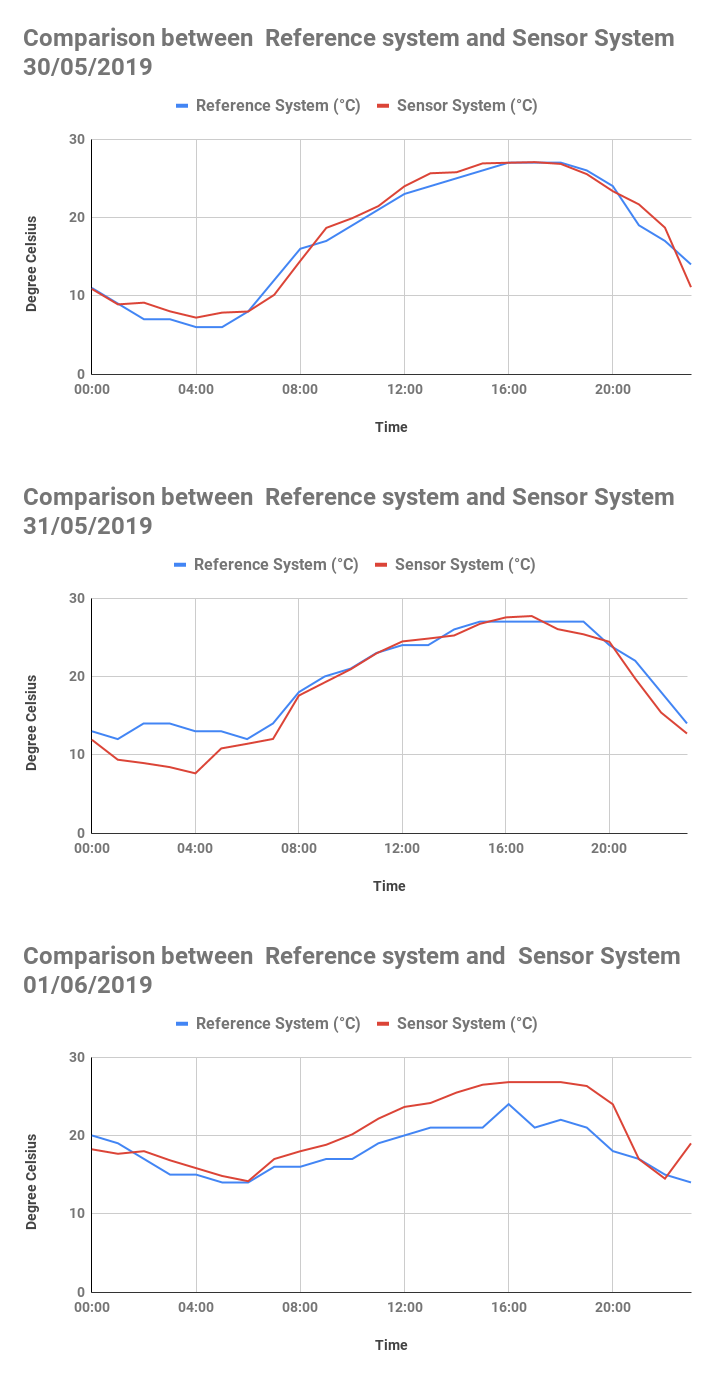
\includegraphics[scale=0.36]{images/figure85tem.png}
    \end{center}
    \caption{Comparison between Temperature values from the sensor system and reference system from 30/05/2019 to 01/06/2019}
  \label{temp}
  
  \end{figure}
  
  
  \begin{figure}[h]
    \begin{center}
    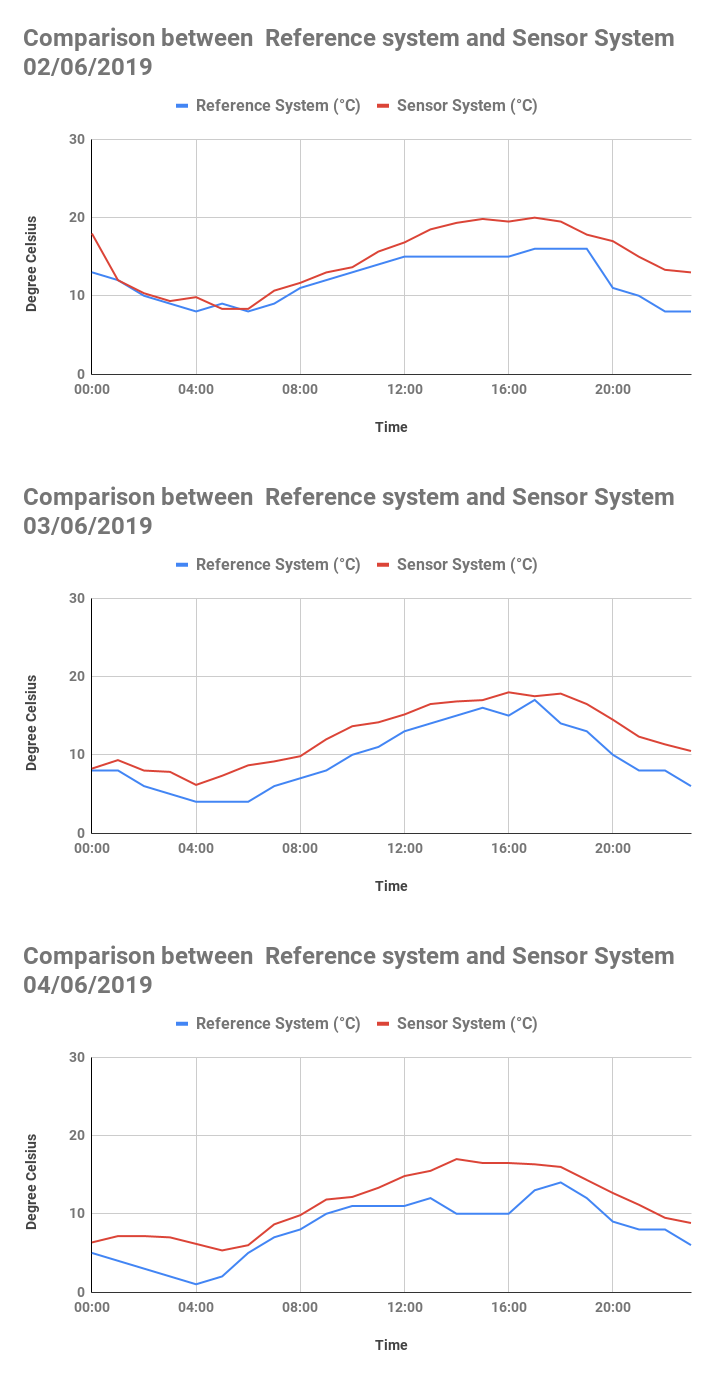
\includegraphics[scale=0.45]{images/figure86tem.png}
    \end{center}
    \caption{Comparison between Temperature values from the sensor system and reference system from 02/06/2019 to 04/06/2019}
    \label{temp1}
  
  \end{figure}



\begin{figure}[h]
  \begin{center}
  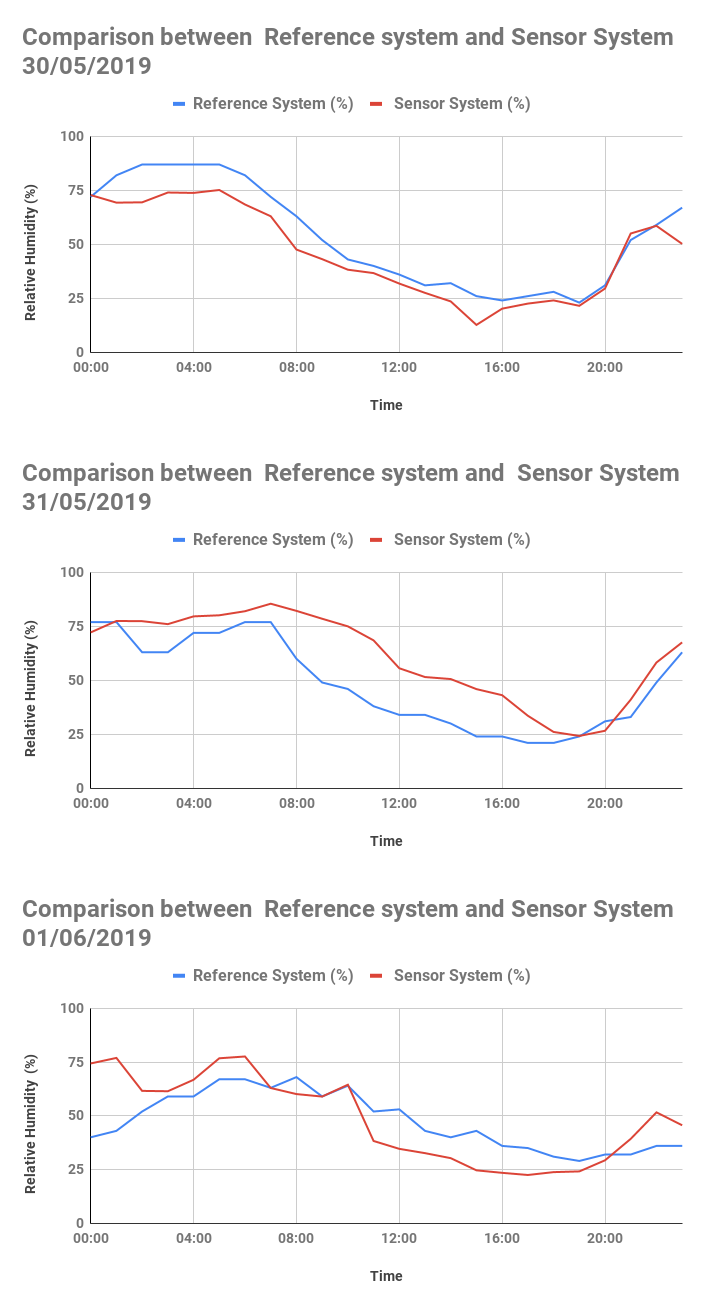
\includegraphics[scale=0.45]{images/figure87hum.png}
  \end{center}
  \caption{Comparison between Humidity values from the sensor system and reference system from 30/05/2019 to 01/06/2019}
\label{hum}

\end{figure}


\begin{figure}[h]
  \begin{center}
  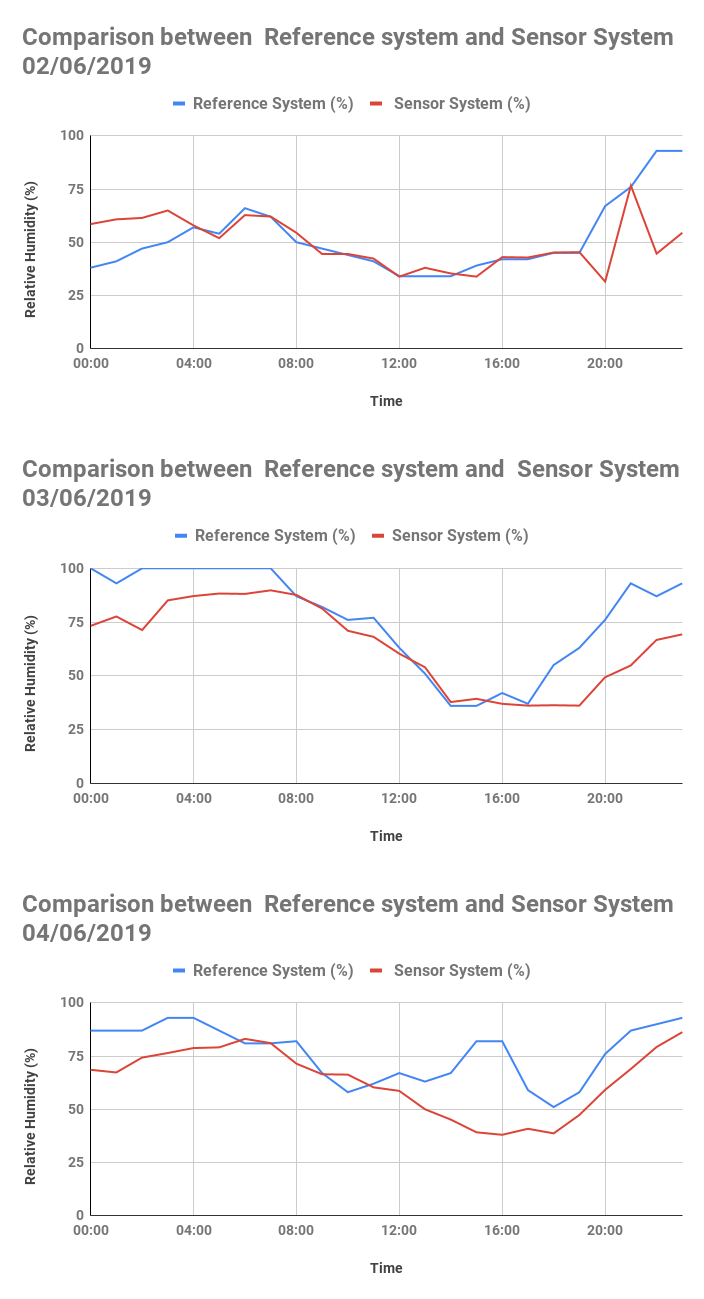
\includegraphics[scale=0.45]{images/figure88hum.png}
  \end{center}
  \caption{Comparison between Humidity values from the sensor system and reference system from 02/06/2019 to 04/06/2019}
  \label{hum1}

\end{figure}



\begin{figure}[h]
  \begin{center}
  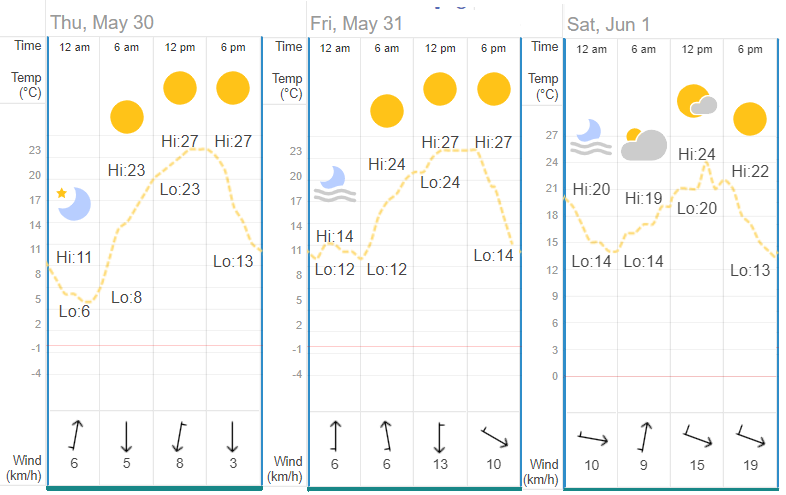
\includegraphics[scale=.90]{images/figure96.png}
  \end{center}
  \caption{Sun graph for Prince George from 30/05/2019 to 01/06/2019  \cite{sunlight} }
\label{sun}

\end{figure}


\begin{figure}[h]
  \begin{center}
  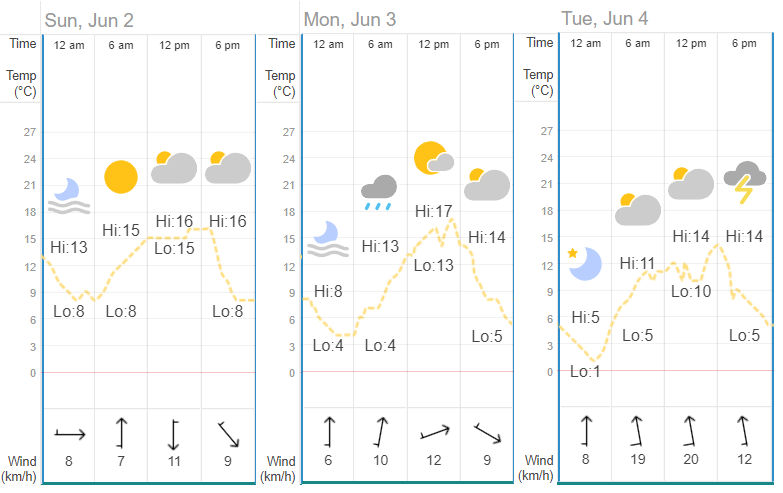
\includegraphics[scale=.90]{images/figure97.png}
  \end{center}
  \caption{Sun graph for Prince George from 02/06/2019 to 04/06/2019  \cite{sunlight} }
  \label{sun1}

\end{figure}
